%%%%%%%%%%%%%%%%%%%%%%%%%%%%%%%%%%%%%%%%%%%%%%%%%%%%%%%%%%%%%%%
%%%%%%%%%%%%%%%%%%%%%%%%%%%%%%%%%%%%%%%%%%%%%%%%%%%%%%%%%%%%%%%

%%%%%%%%%%%%%%%%%%%%%%%%%%%%%%%%%%%%%%%%%%%%%%%%%%%%%%%%%%%%%%%
% Please, use it as a template for your own input, and, please,
% follow carefully the instructions in this document.
%
%%%%%%%%%%%%%%%%%%%%%%%%%%%%%%%%%%%%%%%%%%%%%%%%%%%%%%%%%%%%%%%
\documentclass[11pt]{article}
\usepackage[english]{babel}
\usepackage{xcolor}
\usepackage{hyperref}
\hypersetup{
    colorlinks=true,
    linkcolor=blue,
    allcolors=blue,
    filecolor=blue,      
    urlcolor=blue,
    pdftitle={Overleaf Example},
    pdfpagemode=FullScreen,
    }
\usepackage{amssymb,amsmath,amsfonts,latexsym,graphicx}
\usepackage[utf8]{inputenc}
\usepackage[T1]{fontenc}
\usepackage{lmodern}
\usepackage{tabularx,array,booktabs}
\usepackage[left=2.5cm,right=2.5cm,top=1.5cm,bottom=2.5cm,footnotesep=0.5cm]{geometry}
\usepackage{eso-pic}
\usepackage{tikz}

\setlength{\oddsidemargin}{0.5cm}
\setlength{\textwidth}{15.5cm}
\setlength{\topmargin}{-1.5cm}
\setlength{\textheight}{22cm}   			

\pagestyle{empty}

\begin{document}

% Watermark configuration - UFCG logo on all pages
\AddToShipoutPictureBG{%
    \begin{tikzpicture}[remember picture, overlay]
        \node[opacity=0.15] at (current page.center) {%
            \includegraphics[width=0.3\textwidth]{fig/UFCG_brasao.png}%
        };
    \end{tikzpicture}%
}

\begin{center}
    \Large{\textbf{Nota técnica SKARAB}}
\end{center}

\begin{center}
Rafael A. Batista\\
\vspace{0.1cm}
LABMET \& Unidade Acadêmica de Física - Universidade Federal de Campina Grande, Brasil.\\
\vspace{0.1cm}
{\color{blue}rafael.alves.batista@gmail.com}
\end{center}
% Text of the abstract

\abstract{Esta nota t\'ecnica descreve a implementa\c{c}\~ao, configura\c{c}\~ao e os resultados preliminares da plataforma SKARAB no radiotelesc\'opio BINGO. Utilizando o ecossistema CASPER, a plataforma foi configurada como um analisador de espectro em tempo real para o processamento digital de sinais. Discutimos os desafios de instala\c{c}\~ao, a valida\c{c}\~ao do sistema com diferentes fontes de sinal e a infraestrutura de armazenamento de dados. Os resultados em bancada confirmam a viabilidade da SKARAB para a opera\c{c}\~ao do BINGO, estabelecendo a base para futuras discuss\~oes sobre calibra\c{c}\~ao e estabilidade do sistema.}

\tableofcontents
\newpage

\section{Introdução}

\quad O presente trabalho documenta de forma abrangente a implementação, configuração e validação experimental da plataforma SKARAB como backend digital para o radiotelescópio BINGO (Baryon Acoustic Oscillations from Integrated Neutral Gas Observations). Esta nota técnica representa o registro consolidado das atividades de instrumentação desenvolvidas no âmbito do projeto, integrando conhecimento teórico em processamento digital de sinais, prática de instrumentação científica aplicada à radioastronomia e caracterização de sistemas receptores de micro-ondas.

A plataforma SKARAB (\textbf{S}quare \textbf{K}ilometre \textbf{A}rray \textbf{R}econfigurable \textbf{A}pplication \textbf{B}oard) é uma solução de hardware reconfigurável baseada em FPGA Virtex-7 (XC7VX690T), desenvolvida pela empresa sul-africana Peralex de acordo com as especificações do SKAO-SA. Equipada com conversores analógico-digitais (ADC) de 14 bits operando a 3 GSps e interfaces Ethernet de 40 GbE, a SKARAB oferece capacidade de processamento em tempo real adequada para espectrometria digital de banda larga, requisito fundamental para observações de HI (hidrogênio neutro) na faixa de 980-1260 MHz.

\subsection*{Escopo e Objetivos}

Os objetivos principais desta nota técnica são:

\begin{itemize}
    \item \textbf{Descrição da plataforma SKARAB}: Apresentar as características técnicas do hardware, incluindo a FPGA Virtex-7, os conversores ADC TI ADC32RF45, os módulos mezzanine QSFP+ para transmissão de dados, e a arquitetura de processamento reconfigurável;
    
    \item \textbf{Infraestrutura de software}: Documentar o processo de instalação e configuração do ecossistema CASPER (Collaboration for Astronomy Signal Processing and Electronics Research), incluindo as ferramentas \textit{casperfpga} (Python 2.7), \textit{mlib\_devel} (Python 3.x), MATLAB R2018a, Xilinx Vivado 2019.1 e o fluxo de desenvolvimento de firmware para FPGA;
    
    \item \textbf{Processamento digital de sinais}: Explicar os fundamentos da espectrometria digital implementada na SKARAB, incluindo os conceitos de decimação, conversão digital descendente (DDC), transformada rápida de Fourier (FFT) e acumulação vetorial;
    
    \item \textbf{Desenvolvimento de espectrômetro}: Detalhar o design e implementação do espectrômetro de banda larga operando a 187,5 MHz com 32.768 bins de frequência, descrevendo os blocos funcionais em Simulink e o fluxo de geração de bitstream;
    
    \item \textbf{Caracterização do receptor analógico}: Apresentar as medições de caracterização dos componentes do receptor Uirapuru, incluindo amplificadores de baixo ruído (LNA), filtros passa-banda tipo cavidade, isoladores e acopladores híbridos, documentando parâmetros S ($S_{21}$, $S_{11}$) medidos no Laboratório de Metrologia (LABMET);
    
    \item \textbf{Validação experimental}: Reportar os resultados de testes em bancada e observações com a corneta Uirapuru, incluindo detecção de sinais controlados (RFI intencional com drone), sinais GPS L5 (1176 MHz), trânsitos solares e observações de 24 horas em modo TOD (Time-Ordered Data);
    
    \item \textbf{Infraestrutura de dados}: Descrever o desenvolvimento do sistema de aquisição de dados, incluindo transmissão UDP via 40 GbE, protocolo SPEAD para metadados, geração de arquivos FITS e estratégias de armazenamento em larga escala;
    
    \item \textbf{Estado atual e perspectivas}: Apresentar o status consolidado do projeto, identificando conquistas alcançadas, próximos passos planejados e desafios técnicos em aberto nas áreas de receptor analógico, backend digital e pipeline de dados.
\end{itemize}

\subsection*{Contexto do Projeto BINGO}

Como parte da fase de instrumentação (estágio 0) do projeto BINGO, os trabalhos em torno da SKARAB são fundamentados nos tutoriais e ferramentas disponibilizados pela colaboração CASPER\footnote{\url{https://casper.berkeley.edu}}, uma iniciativa internacional dedicada ao desenvolvimento de sistemas de processamento de sinais para radioastronomia. O ecossistema CASPER fornece bibliotecas de blocos para MATLAB/Simulink, ferramentas de compilação automática (\textit{toolflow}) e frameworks de controle em Python, permitindo o desenvolvimento rápido de sistemas de aquisição e processamento digital de sinais.

Os principais recursos utilizados incluem:

\begin{itemize}
    \item Software em geral: \url{https://casper.berkeley.edu/wiki/Software}
    \item Toolflows e documentação: \url{https://casper-toolflow.readthedocs.io/en/latest/}
    \item Tutoriais: A documentação original (\url{https://casper.berkeley.edu/wiki/Tutorials}) não é atualizada desde 2017, tendo sido migrada para o repositório GitHub da colaboração. Ambas as fontes foram consultadas neste trabalho.
\end{itemize}

\subsection*{Estrutura do Documento}

Esta nota técnica está organizada da seguinte forma:

\begin{itemize}
    \item \textbf{Seção 2 -- Descrição das SKARABs}: Apresenta a arquitetura de hardware da plataforma, incluindo especificações detalhadas da FPGA Virtex-7 XC7VX690T (693.120 células lógicas, 3.600 blocos DSP), dos conversores ADC TI ADC32RF45 (dual-channel, 14-bit, 3 GSps) e dos módulos mezzanine QSFP+ (4$\times$40 GbE). Inclui também uma introdução aos conceitos de FPGA e computação reconfigurável.
    
    \item \textbf{Seção 3 -- Descrição das Atividades}: Detalha a trajetória de desenvolvimento, desde a instalação dos ambientes de software (Ubuntu 16.04, MATLAB, Vivado) até a implementação de espectrômetros funcionais. Aborda os conceitos de decimação e DDC, apresenta o fluxo de trabalho (workflow) para geração de bitstream e programação da FPGA, detalha o tutorial introdutório de familiarização com a SKARAB e descreve o design completo do espectrômetro (Tutorial 4), incluindo os blocos ADC, FFT, cálculo de potência e acumulação vetorial em BRAM. Apresenta os primeiros resultados obtidos em bancada com tons de CW e fontes de ruído.
    
    \item \textbf{Seção 4 -- Status Atual do Trabalho}: Documenta o estado atual do protótipo do receptor analógico Uirapuru, apresentando medições de caracterização de componentes (LNA WanTcom modelo WBA0913AS com ganho de 38 dB, filtro passa-banda de cavidade 980-1260 MHz, isolador UIY 3434A960T1260SF, acoplador híbrido). Reporta os resultados de observações experimentais, incluindo testes com transmissor em drone (detecção do terceiro harmônico em 1200 MHz), observações de sinais GPS L5 e trânsitos solares, e waterfall plots de 24 horas mostrando a passagem de satélites. Apresenta uma tabela consolidada de conquistas, próximos passos e desafios nas três frentes principais: receptor analógico, backend SKARAB e infraestrutura de dados FITS.
    
    \item \textbf{Apêndices}: Fornecem instruções detalhadas e reproduzíveis para instalação do ambiente \textit{casperfpga} (Python 2.7) e do ambiente \textit{mlib\_devel} (MATLAB R2018a, Vivado 2019.1, Python 3.x), incluindo resolução de dependências, configuração de ambientes virtuais, compilação de ferramentas auxiliares e configuração de rede 40 GbE.
\end{itemize}

Esta documentação serve como referência técnica para a operação da plataforma SKARAB no contexto do BINGO e estabelece a base para futuras discussões sobre calibração, estabilidade de sistema, sincronização multi-placa e estratégias de mitigação de RFI (Radio Frequency Interference).

\section{Descrição das SKARABs}

\quad A SKARAB (\textbf{S}quare \textbf{K}ilometre \textbf{A}rray \textbf{R}econfigurable \textbf{A}pplication \textbf{B}) é uma plataforma de hardware de aquisição e processamento de dados baseada em FPGA (Field Programmable Gate Array), utilizando um Virtex-7 (XC7VX690T). Desenvolvida pela empresa sul-africana Peralex de acordo com as especificações do SKAO-SA, a SKARAB é ideal para aplicações em radioastronomia \cite{melis2024skarab} e otimizada para processamento digital de sinais de alto desempenho, possuindo mais de 690.000 células lógicas, 3.600 blocos DSP e 53 Mb de memória RAM.

Ela integra um conversor analógico-digital (ADC) de 14 bits com taxa de amostragem de 3 GSps, permitindo amostragem livre de aliasing até 1,5 GHz, adequada para o processamento simultâneo e preciso de múltiplas faixas de frequência. O ADC suporta conexão com um conversor digital descendente (DDC) de banda dupla, que inclui até três osciladores numericamente controlados (NCOs) de 16 bits por DDC, possibilitando saltos de frequência coerentes em fase.

Além do ADC, a SKARAB possui suporte a periféricos Mezzanine para armazenamento e transmissão de dados. Um exemplo é o módulo Mezzanine Ethernet, que inclui quatro interfaces QSFP+ (Quad Small Form-factor Pluggable Plus), cada uma com taxa de até 40 GbE, resultando em largura de banda agregada de até 160 Gbps. A plataforma oferece espaço para quatro placas Mezzanine, cada uma com interface para 16 transceptores seriais de alta velocidade (10~Gb/s). Atualmente, existem três placas mezzanine para a SKARAB disponíveis no mercado: 
\begin{itemize}
    \item Módulo Mezzanine QSFP+ com quatro interfaces Ethernet de 40 Gb;
    \item Módulo Hybrid Memory Cube (HMC) com alta largura de banda de memória e capacidade de 4 GB por módulo;
    \item Placa Mezzanine ADC compatível com a interface mezzanine SKARAB, fornecendo dois chips ADC TI AD32RF45 dual 3 GSPS de 14 bits com DDC, para quatro canais A/D por placa.
\end{itemize}

Atualmente, a placa SKARAB do projeto BINGO está equipada com um único Módulo Mezzanine QSFP+ e dois Módulos Mezzanine ADC, não incluindo um Módulo Hybrid Memory Cube.

\subsection{Introdução à FPGA e Computação Reconfigurável}

\quad Um FPGA (Field Programmable Gate Array) é um circuito integrado digital cuja principal característica é poder ser configurado pelo usuário após a fabricação. Diferente de chips com funções fixas, como microcontroladores ou ASICs, o FPGA é composto por uma matriz de blocos lógicos programáveis, memórias, e interconexões reconfiguráveis, permitindo implementar circuitos digitais personalizados em nível de hardware.

Ele é considerado reprogramável porque sua funcionalidade não é determinada permanentemente. O comportamento do FPGA é definido por um arquivo de configuração chamado bitstream, que contém os dados necessários para ajustar o estado interno dos blocos lógicos e das conexões entre eles.

Durante a programação, o bitstream é carregado na memória interna do FPGA (geralmente SRAM), configurando as portas lógicas, roteamentos e registradores de acordo com o circuito descrito em uma linguagem de descrição de hardware (como VHDL ou Verilog). Ao alterar o bitstream, é possível mudar completamente a função do hardware, por exemplo, transformar um processador digital em um filtro de sinais, e vice-versa — tudo no mesmo dispositivo físico.

Assim, o FPGA combina a flexibilidade do software com o desempenho do hardware dedicado, sendo amplamente usado em aplicações que exigem alto desempenho e possibilidade de atualização ou prototipagem rápida.

\subsubsection{FPGA da SKARAB: Virtex-7 XC7VX690T-2FFG1927C}

O \textbf{Virtex-7 XC7VX690T-2FFG1927C} é um FPGA de alto desempenho da família Virtex-7 da AMD (anteriormente Xilinx), projetado para aplicações que exigem alta capacidade de lógica, largura de banda elevada e eficiência energética. Fabricado utilizando tecnologia de processo de 28 nm HPL (High-Performance, Low-Power) com tecnologia de porta metálica de alto-k (HKMG), este dispositivo oferece uma solução robusta para sistemas de processamento de sinais, redes de alta velocidade e prototipagem de ASICs.

\subsection*{Especificações Principais}
\begin{itemize}
    \item \textbf{Células Lógicas}: 693.120
    \item \textbf{Módulos Lógicos Adaptáveis (ALMs)}: 108.300
    \item \textbf{Memória Embutida}: 51,68 Mbit
    \item \textbf{Número de I/Os}: 600
    \item \textbf{Taxa de Dados Máxima}: 28,05 Gb/s
    \item \textbf{Número de Transceptores}: 80
    \item \textbf{Frequência Máxima de Operação}: 640 MHz
    \item \textbf{Tensão de Alimentação}: 0,97 V a 1,03 V
    \item \textbf{Temperatura de Operação}: 0°C a 85°C
    \item \textbf{Pacote}: FCBGA-1927 (45 mm x 45 mm)
\end{itemize}

\subsection*{Arquitetura e Recursos}
\begin{itemize}
    \item \textbf{LUTs de 6 Entradas}: Utilizadas para lógica avançada e memória distribuída.
    \item \textbf{Memória RAM Distribuída}: 10.888 Kbit.
    \item \textbf{Memória RAM de Bloco (BRAM)}: 52.920 Kbit.
    \item \textbf{Módulos de Gerenciamento de Clock (CMT)}: Inclui PLLs e MMCMs para gerenciamento preciso de clock.
    \item \textbf{XADC Dual de 12 bits}: Conversores analógico-digital integrados com sensores térmicos e de alimentação.
\end{itemize}

\subsection*{Aplicações Típicas}
\begin{itemize}
    \item Redes de alta velocidade (10G a 100G).
    \item Sistemas de radar portáteis.
    \item Prototipagem de ASICs.
    \item Processamento de sinais de alta performance.
    \item Aplicações em comunicações ópticas e de rádio frequência.
\end{itemize}

\subsection*{Vantagens}
\begin{itemize}
    \item \textbf{Alta Densidade Lógica}: Até 2 milhões de células lógicas em variantes superiores.
    \item \textbf{Baixo Consumo de Energia}: Até 50\% mais eficiente energeticamente em comparação com soluções de múltiplos chips.
    \item \textbf{Alta Largura de Banda Serial}: Suporte a transceptores de até 28,05 Gb/s.
    \item \textbf{Arquitetura Escalável}: Facilita a migração de designs da família Virtex-6.
\end{itemize}

Para especificações completas e datasheet, visite: \url{https://www.xilinx.com/support/documentation/data_sheets/ds183_Virtex_7_Data_Sheet.pdf}.


\subsection{Mezzanine ADC da SKARAB: TI ADC32RF45}

\quad ADC32RF45 é um conversor analógico-digital (ADC) de alto desempenho, dual-channel, com 14 bits de resolução, otimizado para aplicações de amostragem RF de banda larga, como comunicações 5G, radar e guerra eletrônica. Cada canal suporta taxas de amostragem de até 3,0 GSPS e frequências de entrada de até 4,0 GHz.

\subsection*{Principais Especificações}
\begin{itemize}
    \item Resolução: 14 bits
    \item Taxa de Amostragem: 3,0 GSPS por canal
    \item Frequência de Entrada: DC a 4,0 GHz
    \item Tensão de Entrada: 1,35 Vpp diferencial
    \item Densidade Espectral de Ruído: –155 dBFS/Hz
    \item Jitter de Abertura (Aperture Jitter): 90 fs
    \item Isolamento entre Canais: 95 dB @ 1,8 GHz
    \item Consumo de Energia: 3,2 W por canal @ 3,0 GSPS
    \item Pacote: VQFN de 72 pinos (10 mm × 10 mm)
\end{itemize}

\subsection*{Desempenho}
\begin{itemize}
    \item SNR: 60,9 dBFS @ 900 MHz, 58,8 dBFS @ 1,78 GHz
    \item SFDR: 67 dBc (HD2, HD3) @ 900 MHz, 66 dBc @ 1,78 GHz
    \item Pior Spur SFDR: 77 dBc @ 900 MHz, 75 dBc @ 1,78 GHz
\end{itemize}

\subsection*{Conversor Digital Descendente (DDC)}
\begin{itemize}
    \item Até 4 DDCs por canal, modo dual-band
    \item 3 NCOs independentes de 16 bits por DDC
    \item Detectores de pico e RMS integrados
    \item Terminação de entrada e proteção contra sobretensão
\end{itemize}

\subsection*{Interface \& Sincronização}
\begin{itemize}
    \item JESD204B Subclasse 1, latência determinística
    \item 4 lanes por canal, até 12,5 Gbps por lane
    \item Sincronização multi-chip para sistemas phased-array
\end{itemize}

\subsection*{Avaliação \& Desenvolvimento}
\begin{itemize}
    \item ADC32RF45EVM com gerador de clock LMK04828 onboard
    \item Suporta clock externo e interface JESD204B
    \item GUI para configuração e controle
\end{itemize}

\subsection*{Aplicações}
\begin{itemize}
    \item Comunicações de banda larga (5G e além)
    \item Sistemas de radar (phased-array, SAR)
    \item Guerra eletrônica e inteligência de sinais
    \item Testes e medições de sinais de alta frequência
\end{itemize}

Para especificações completas e datasheet, visite: \url{https://www.ti.com/product/ADC32RF45}.



\subsection{Descrição do setup de medidas}






\section{Descrição das atividades}

\subsection{Testes do fabricante}

\quad Os únicos testes disponíveis para o manuseio da placa SKARAB encontram-se nos tutoriais da CASPER, que não recebem atualizações desde 2017. Entre esses tutoriais, destacam-se o tutorial introdutório (tutorial 1), que orienta a criação de um design de blocos simples para a soma de valores de registradores e o uso de blocos contadores.
Em seguida, há o tutorial voltado à interface QSFP+ Ethernet (tutorial 2), que aborda sua configuração e manipulação.
Por fim — e de maior relevância — encontra-se o tutorial do espectrômetro (tutorial 4 e 5), no qual o design de blocos inclui um ADC responsável pela captura de dados para processamento digital de sinais, culminando na plotagem do espectro obtido. Para acessar os tutoriais da CASPER, click no seguinte link\footnote{https://casper-toolflow.readthedocs.io/projects/tutorials/en/latest/}.

\subsection{Instalação de pacotes básicos}

\quad A implementação da plataforma SKARAB e a aquisição de dados foram realizadas em um ambiente Python. Inicialmente, utilizou-se o sistema operacional Ubuntu 16.04 LTS, uma vez que esta era a única versão compatível com os softwares necessários para a descrição do hardware implementado na SKARAB. A identificação e compreensão dos requisitos essenciais para a correta configuração dos ambientes representaram um desafio significativo, demandando vários meses de trabalho contínuo e análise detalhada, em razão da escassa documentação disponibilizada pela colaboração CASPER. Ao final desse processo, foi possível mapear com sucesso as dependências dos pacotes \textit{casperfpga} (veja apêndice \ref{appendix:casperfpga}) e \textit{mlib\_devel} (veja apêndice \ref{appendix:mlib_devel}), estabelecendo uma base sólida para o desenvolvimento e operação da plataforma.

\subsection{A questão da decimação}

\quad A decimação, em processamento de sinal digital (DSP), consiste em reduzir a taxa de amostragem de um sinal, isto é, diminuir o número de amostras por segundo. A decimação é amplamente empregada em sistemas de rádio definido por software (SDR) e aplicações de comunicação digital, pois permite concentrar o processamento apenas na banda de interesse, reduzindo significativamente a quantidade de dados e o custo computacional. Esse processo afeta diretamente o comprimento (ou largura) de banda do espectro analisado, uma vez que a largura de banda máxima de um sinal digital é proporcional à sua frequência de amostragem.

Na placa SKARAB, a decimação é implementada digitalmente dentro do bloco DDC (Digital Downconverter), executado em FPGA. Esse bloco combina operações de translação de frequência (mixagem digital), filtragem e redução da taxa de amostragem, permitindo isolar e extrair sub-bandas específicas do sinal de entrada de 3 GHz com elevada flexibilidade. A placa utiliza ADCs operando a uma taxa de amostragem de 3 GHz; entretanto, no modo DDC, os fatores de decimação programáveis disponíveis no design de blocos do Simulink são de 4, 8, 16, 32, entre outros. Assim, o maior comprimento de banda alcançável é de aproximadamente 750 MHz, correspondente ao fator de decimação igual a 4.

No contexto do projeto BINGO, um fator de decimação igual a 8 mostra-se adequado para o comprimento de banda de interesse (ver linha 7 da Tabela \ref{tab1}). Esse fator resulta em uma largura de banda de 375 MHz, valor que pode ser ajustado conforme a taxa de amostragem selecionada para o ADC. A Tabela \ref{tab1} apresenta de forma completa a relação entre a taxa de amostragem de saída, a taxa de amostragem do ADC e do FPGA, bem como os fatores de decimação e de reamostragem (resampler) empregados no sistema.

\begin{table}[htbp]
\centering
\caption{Taxas de Amostragem (\textbf{TA}) disponíveis no ADC da SKARAB.}
\label{tab1}
\small
\begin{tabular}{|l|c|c|c|c|c|c|}
\hline
\textbf{Ref} & \textbf{TA ADC} & \textbf{Decim. ADC} & \textbf{Decim. FPGA} & \textbf{Resamp.} & \textbf{TA Out} & \textbf{Tipo Out} \\ \hline
1.&2800& 1& 1 & 1 & 2800 & Real \\ \hline
2.&2560& 1& 1 & 1 & 2560 & Real \\ \hline
3.&2560& 1& 1 & 0.8 & 2048 & Real \\ \hline
4.&3000& 4& 1 & 1 & 750 & Complexo \\ \hline
5.&2560& 4& 1 & 1 & 640 & Complexo \\ \hline
6.&2560& 4& 1 & 0.8 & 512 & Complexo \\ \hline
7.&3000& 8& 1 & 1 & 375 & Complexo \\ \hline
8.&2560& 8& 1 & 1 & 320 & Complexo \\ \hline
9.&2560& 8& 1 & 0.8 & 256 & Complexo \\ \hline
10.&3000& 16& 1 & 1 & 187.5 & Complexo \\ \hline
11.&2560& 16& 1 & 1 & 160 & Complexo \\ \hline
12.&2560& 16& 1 & 0.8 & 128 & Complexo \\ \hline
13.&3000& 16& 2 & 1 & 93.75 & Complexo \\ \hline
14.&2560& 16& 2 & 1 & 80 & Complexo \\ \hline
15.&2560& 16& 2 & 0.8 & 64 & Complexo \\ \hline
16.&3000& 16& 4 & 1 & 46.875 & Complexo \\ \hline
17.&2560& 16& 4 & 1 & 40 & Complexo \\ \hline
18.&2560& 16& 4 & 0.8 & 32 & Complexo \\ \hline
19.&3000& 16& 8 & 1 & 23.4375 & Complexo \\ \hline
20.&2560& 16& 8 & 1 & 20 & Complexo \\ \hline
21.&2560& 16& 8 & 0.8 & 16 & Complexo \\ \hline
\end{tabular}
\end{table}



\subsection{Requisitos de Software e Instalação}

\quad Para o desenvolvimento e operação da plataforma SKARAB, é necessária uma infraestrutura de software específica, composta por ferramentas proprietárias e pacotes de código aberto mantidos pela colaboração CASPER. A Tabela \ref{tab:requirements} resume os principais requisitos de software e suas respectivas versões.

\begin{table}[htbp]
\caption{Requisitos de software para a plataforma SKARAB.}
\begin{center}
\begin{tabular}{|l|l|}
\hline
\textbf{Software / Pacote} & \textbf{Versão Requerida} \\ \hline
Sistema Operacional & Ubuntu 16.04 LTS \\ \hline
MATLAB & R2018a \\ \hline
Xilinx Vivado & 2019.1 \\ \hline
Python (Controle) & 2.7 (Ambiente \textit{casperfpga}) \\ \hline
Python (Toolflow) & 3.x (Ambiente \textit{mlib\_devel}) \\ \hline
\textit{casperfpga} & Última versão compatível (Python 2.7) \\ \hline
\textit{mlib\_devel} & Master branch (compatível com Vivado 2019.1) \\ \hline
\end{tabular}
\label{tab:requirements}
\end{center}
\end{table}

A instalação detalhada desses componentes é apresentada nos apêndices desta nota técnica. O Apêndice \ref{appendix:casperfpga} detalha a configuração do ambiente Python 2.7 e a instalação do pacote \textit{casperfpga}, essencial para a comunicação e programação da placa. O Apêndice \ref{appendix:mlib_devel} descreve o processo de instalação do MATLAB, Vivado e do toolflow \textit{mlib\_devel}, necessários para a criação de novos firmwares.

\subsection{Geração de Bitstream e Programação da FPGA}

\quad O processo de transformar um modelo matemático em um hardware funcional na FPGA da SKARAB envolve duas etapas principais: a geração do arquivo de configuração (bitstream) e a transferência deste para a placa. \textbf{É importante ressaltar que este procedimento é geral para qualquer tutorial ou design desenvolvido para a placa}, consistindo nos passos fundamentais de compilação e implementação (\textit{deployment}) do \textit{bitstream}.

\subsubsection{Geração de Bitstream}

A geração do bitstream é realizada através do ambiente MATLAB/Simulink utilizando o toolflow \textit{mlib\_devel}. O fluxo de trabalho segue os seguintes passos:
\begin{enumerate}
    \item \textbf{Modelagem}: O design do firmware é construído no Simulink utilizando blocos da biblioteca CASPER e do Xilinx System Generator.
    \item \textbf{Configuração}: Definição do hardware alvo (SKARAB) e parâmetros de clock.
    \item \textbf{Síntese}: O comando \texttt{jasper} no MATLAB inicia o processo de compilação automática, que utiliza o Vivado em segundo plano.
    \item \textbf{Arquivo FPG}: Ao final, um arquivo \texttt{.fpg} é gerado, contendo o bitstream e metadados dos registros.
\end{enumerate}

\begin{figure}[!htb]
\centering
\includegraphics[width=0.8\textwidth]{fig/skarab_workflow.png}
\caption{Fluxo de trabalho geral para a plataforma SKARAB, aplic\'avel a qualquer design e tutorial. O processo abrange desde a modelagem em Simulink at\'e a gera\c{c}\~ao do bitstream e programa\c{c}\~ao da FPGA.}
\label{fig:SkarabWorkflow}
\end{figure}

\section{Tutorial de Introdução ao SKARAB}

\quad Este tutorial, baseado na documentação oficial do CASPER\footnote{\url{https://casper-toolflow.readthedocs.io/projects/tutorials/en/latest/tutorials/skarab/tut_intro.html}}, descreve os passos fundamentais para criar, simular e compilar um design básico para a plataforma SKARAB. O objetivo é familiarizar o usuário com o fluxo de trabalho (\textit{toolflow}) e a integração entre MATLAB/Simulink e o hardware.

\subsection{Configuração do Ambiente e Criação do Modelo}

O primeiro passo é iniciar o MATLAB através do comando \texttt{startsg}, que carrega as bibliotecas CASPER e Xilinx necessárias. No Simulink, cria-se um novo modelo (arquivo \texttt{.slx}), observando restrições como evitar espaços ou letras maiúsculas no nome do arquivo e caminhos.

\begin{figure}[!htb]
\centering
\includegraphics[width=0.6\textwidth]{fig/tut_platform.png}
\caption{Seleção da plataforma SKARAB no bloco \textit{XPS Config} da biblioteca CASPER.}
\label{fig:tut_platform}
\end{figure}

Deve-se adicionar o bloco \textit{System Generator} e o bloco de configuração da plataforma (\textit{XPS Config}), conforme mostrado na Fig. \ref{fig:tut_platform}. Para a SKARAB, é essencial configurar o clock de IP do usuário (\textit{User IP Clock Source}) para \texttt{sys\_clk} em designs experimentais iniciais.

\subsection{Integração de Blocos e Lógica de Design}

Cada design SKARAB deve conter um core de Ethernet para comunicação. Recomenda-se utilizar o template oficial que já inclui o core de 40GbE configurado (Fig. \ref{fig:tut_core}).

\begin{figure}[!htb]
\centering
\includegraphics[width=0.45\textwidth]{fig/tut_core.png}
\caption{Subsistema de comunicação Ethernet 40GbE integrado ao modelo.}
\label{fig:tut_core}
\end{figure}

O tutorial propõe dois exercícios práticos fundamentais:
\begin{enumerate}
    \item \textbf{LED Piscante}: Utiliza um contador de 27 bits, onde o bit mais significativo (MSB) é extraído via bloco \textit{Slice} e enviado a um bloco \textit{GPIO} mapeado para os LEDs da SKARAB (Fig. \ref{fig:tut_led_circuit}).
    \item \textbf{Operação de Soma}: Demonstra o uso de registros de software (\textit{Software Registers}) para controle bidirecional. Registros "\textit{From Processor}" fornecem dados para um bloco \textit{AddSub}, e um registro "\textit{To Processor}" permite a leitura do resultado (Fig. \ref{fig:tut_adder_circuit}).
\end{enumerate}

\begin{figure}[!htb]
\centering
\begin{minipage}{0.48\textwidth}
    \centering
    \includegraphics[width=\textwidth]{fig/tut_led_circuit.png}
    \caption{L\'ogica para controle de LED.}
    \label{fig:tut_led_circuit}
\end{minipage}
\hfill
\begin{minipage}{0.48\textwidth}
    \centering
    \includegraphics[width=\textwidth]{fig/tut_adder_circuit.png}
    \caption{Circuito de soma via software.}
    \label{fig:tut_adder_circuit}
\end{minipage}
\end{figure}

\subsection{Simula\c{c}\~ao e Compila\c{c}\~ao}

O design pode ser simulado com precis\~ao de clock no Simulink. Ap\'os validar o comportamento, executa-se o comando \texttt{jasper} no prompt do MATLAB. Este processo invoca o compilador da Xilinx e o Vivado para realizar a s\'intese e roteamento (Fig. \ref{fig:tut_compile}), gerando o arquivo \textit{fpg} final na pasta \texttt{outputs}.

\begin{figure}[!htb]
\centering
\includegraphics[width=0.45\textwidth]{fig/tut_compile.png}
\caption{Processo de compila\c{c}\~ao autom\'atica via \textit{toolflow}.}
\label{fig:tut_compile}
\end{figure}

\subsection{Programação e Interação via Python}

A programação da FPGA é realizada através da biblioteca \texttt{casperfpga}. O código abaixo ilustra o procedimento básico de carregamento do firmware e interação com os registros de hardware:

\begin{verbatim}
import casperfpga
# Conexão com a placa
fpga = casperfpga.CasperFpga('10.42.0.201')
# Programação do bitstream
fpga.upload_to_ram_and_program('skarab_tut_intro.fpg')
# Manipulação de registros de software
fpga.write_int('reg_a', 123)
fpga.write_int('reg_b', 456)
resultado = fpga.read_int('sum_a_b')
\end{verbatim}
\subsubsection{Programação da FPGA}

Uma vez gerado o arquivo \texttt{.fpg}, a programação da SKARAB é feita via rede Ethernet (40GbE) utilizando a biblioteca Python \textit{casperfpga}. O procedimento comum realizado no ambiente \textit{IPython} consiste em:
\begin{enumerate}
    \item Importar a biblioteca: \texttt{import casperfpga}.
    \item Conectar à placa: \texttt{fpga = casperfpga.CasperFpga('IP\_DA\_SKARAB')}.
    \item Carregar o firmware: \texttt{fpga.upload\_to\_ram\_and\_program('nome\_do\_arquivo.fpg')}.
\end{enumerate}
Este processo configura instantaneamente a FPGA com o novo design, permitindo o início imediato da aquisição ou processamento de dados.



\subsection{Espectr\^ometro (Tutorial 4)}

\quad Um espectr\^ometro digital converte sinais do dom\'inio do tempo para o dom\'inio da frequ\^encia, geralmente utilizando o algoritmo de Transformada R\'apida de Fourier (FFT). No contexto do BINGO, o design do espectr\^ometro deve equilibrar a resolu\c{c}\~ao temporal (necess\'aria para detectar eventos r\'apidos) e a resolu\c{c}\~ao espectral (para mapeamento de HI). Esta se\c{c}\~ao detalha os blocos fundamentais do design do espectr\^ometro de banda larga desenvolvido no ecossistema CASPER para a SKARAB.

\subsubsection{Digitaliza\c{c}\~ao (ADC)}

\quad O primeiro passo \'e a digitaliza\c{c}\~ao do sinal anal\'ogico. O bloco \texttt{skarab\_adc} (Fig.~\ref{fig:tut_spec_adc}) opera a uma taxa de amostragem de 3,0~GHz com um fator de decima\c{c}\~ao interno de 4, resultando em uma taxa efetiva de amostragem de 750~MHz. O sinal \'e quantizado em 16 bits (formato \texttt{fix\_16\_15}), representando valores entre -1 e 1. A largura de banda total dispon\'ivel (Nyquist) \'e de 375~MHz.

\begin{figure}[!htb]
\centering
\includegraphics[width=0.8\textwidth]{fig/tut_spec_adc_highres.png}
\caption{Bloco de interface e par\^ametros do ADC da SKARAB (\texttt{skarab\_adc4x3g\_14}).}
\label{fig:tut_spec_adc}
\end{figure}

\subsubsection{Transformada de Fourier (FFT)}

\quad O bloco \texttt{fft} (Fig.~\ref{fig:tut_spec_fft}) \'e o n\'ucleo do processamento. Ele recebe fluxos complexos demultiplexados do ADC. Para a SKARAB, o design utiliza um FFT complexo projetado para processar amostras em paralelo, permitindo que o sistema opere em tempo real na frequ\^encia de clock da FPGA (187,5~MHz).

\begin{figure}[!htb]
\centering
\includegraphics[width=0.8\textwidth]{fig/tut_spec_fft_highres.png}
\caption{Par\^ametros de configura\c{c}\~ao do bloco FFT (\textit{Size of FFT}: $2^{12} = 4096$ pontos).}
\label{fig:tut_spec_fft}
\end{figure}

\subsubsection{C\'alculo de Pot\^encia e Acumula\c{c}\~ao}

\quad Ap\'os a FFT, as componentes s\~ao enviadas para blocos de pot\^encia (\texttt{power}, Fig.~\ref{fig:tut_spec_power}), que calculam o quadrado da magnitude ($P = re^2 + im^2$). 

\begin{figure}[!htb]
\centering
\includegraphics[width=0.6\textwidth]{fig/tut_spec_power_highres.png}
\caption{Implementa\c{c}\~ao do c\'alculo de pot\^encia no domínio digital.}
\label{fig:tut_spec_power}
\end{figure}

\quad Para reduzir a taxa de dados e melhorar o sinal-ru\'ido, os espectros s\~ao integrados temporalmente no bloco \texttt{simple\_bram\_vacc} (Fig.~\ref{fig:tut_spec_vacc}). Os dados acumulados s\~ao armazenados em mem\'orias \texttt{BRAM} (\texttt{mem1}), que s\~ao lidas via Python.

\begin{figure}[!htb]
\centering
\includegraphics[width=0.8\textwidth]{fig/tut_spec_vacc_highres.png}
\caption{Acumulador vetorial em BRAM e registro de mem\'oria para leitura de dados.}
\label{fig:tut_spec_vacc}
\end{figure}


\subsection{Resultados}

\quad As primeiras medições usando a SKARAB foram conduzidas no Laboratório de Metrologia (LABMET) em Campina Grande - PB. O primeiro espectro obtido, ilustrado na Fig.~\ref{fig:SKARAB_first_time}, foi gerado com decimação 32, o que resulta em um comprimento de banda de 93,75 MHz, centrado em 900 MHz. A configuração básica usada para testes usando a SKARAB está na Fig.\ref{fig:Configuration}, composta por: (1) gerador de sinal, (2) SKARAB ADC, (3) fonte de ruído, (4) relógio atômico de rubídio com GPS e (5) analisador de espectro auxiliar.

\begin{figure}[!htb]
\centering
\includegraphics[scale=0.6]{fig/SKARAB_first_time.png}
\caption{Primeiro espectro obtido pela SKARAB no LABMET.}
\label{fig:SKARAB_first_time}
\end{figure}

\begin{figure}[!htb]
\centering
\includegraphics[scale=0.4]{fig/aparato (1).jpg}
\caption{Configuração experimental utilizada nos testes da placa SKARAB, composta por: (1) gerador de sinal, (2) SKARAB ADC, (3) fonte de ruído, (4) relógio atômico de rubídio com GPS e (5) analisador de espectro auxiliar.}
\label{fig:Configuration}
\end{figure}

\begin{figure}[!htb]
\centering
\includegraphics[scale=0.5]{fig/spectrum_ns (1).jpg}
\caption{Espectro e waterfall de um sinal contínuo (tom) em 908 MHz com potência de -90 dBm. Após um determinado tempo da inicialização, foi adicionada uma fonte de ruído para observação do efeito sobre o sinal.}
\label{fig:Paper}
\end{figure}

\subsection{O espectrômetro do BINGO e desafios}

    \quad No desenvolvimento do backend digital para o projeto BINGO, a placa SKARAB foi configurada com sucesso para operar como um espectrômetro em tempo real com largura de banda de 187,5~MHz e resolu\c{c}\~ao de 32.768 bins de frequ\^encia. Esta configura\c{c}\~ao baseia-se no \textit{toolflow} CASPER, integrando blocos de FFT (\textit{Fast Fourier Transform}) de alto desempenho e acumuladores vetoriais. A valida\c{c}\~ao do sistema incluiu a identifica\c{c}\~ao da faixa din\^amica livre de esp\'urios (SFDR) e a verifica\c{c}\~ao da integridade do sinal em condi\c{c}\~oes de laborat\'orio.

    Entretanto, a implementa\c{c}\~ao revelou desafios t\'ecnicos significativos. A sincroniza\c{c}\~ao do \textit{clock} de amostragem entre o ADC e o processamento na FPGA exige um controle rigoroso de fase e baixos n\'iveis de \textit{jitter} para evitar degrada\c{c}\~ao na sensibilidade do instrumento. Outro ponto cr\'itico \'e o gerenciamento da alta taxa de transfer\^encia de dados via portas 40~GbE. Em regimes de 187,5~MHz, o fluxo de pacotes UDP deve ser otimizado para evitar perdas ou \textit{overflow} nos \textit{buffers} de recep\c{c}\~ao do servidor de aquisi\c{c}\~ao.

    Os pr\'oximos passos para o espectr\^ometro incluem a expans\~ao da largura de banda para 375~MHz (utilizando dual-ADC) e a redu\c{c}\~ao do n\'umero de bins para 8.192 para otimizar o uso de recursos de mem\'oria BRAM na FPGA. Al\'em disso, estamos desenvolvendo blocos de IP para o gerenciamento de metadados via protocolo SPEAD, garantindo a rastreabilidade temporal dos dados atrav\'es de \textit{timestamps} de alta precis\~ao sincronizados via sinal PPS (\textit{Pulse Per Second}).

No que diz respeito ao receptor analógico, a corneta Uirapuru foi montada e testada, e a caracterização do amplificador de baixo ruído (LNA) e dos filtros já foi concluída.

Os próximos passos envolvem aprimorar as medições de temperatura de ruído, refinar os métodos de calibração e realizar testes de estabilidade uma vez integrado ao sistema SKARAB.

Os principais desafios estão relacionados à mitigação das flutuações e instabilidades de ganho por meio de técnicas como os radiômetros Dicke e de pseudocorrelação, bem como garantir a estabilidade e o desempenho de longo prazo do receptor.

O objetivo principal é usar os módulos ADC do SKARAB para digitalizar quatro entradas de RF cada—duas polarizações ortogonais e duas cargas de referência ColFET—enquanto empregamos a comutação Dicke para reduzir as flutuações de ganho.

No que diz respeito à aquisição de dados e geração de arquivos FITS, uma estrutura de cabeçalho FITS já foi projetada, e os dados de espectro foram armazenados com sucesso no formato FITS.Os próximos passos visam incorporar o suporte completo a metadados via pacotes UDP (por exemplo, tempo de sincronização, marcações temporais (timestamps), contadores de heap e de pacotes), bem como a caracterização da temperatura do sistema ($T_{sys}$) e da temperatura de carga de calibração ($T_{cal}$).Os principais desafios incluem o desenvolvimento de software capaz de integrar dados ordenados por tempo (TOD), metadados SPEAD e marcações temporais de alta precisão em arquivos FITS, juntamente com o estabelecimento de um sistema de banco de dados para o gerenciamento de dados em grande escala.

\begin{table}[h!]
\centering
\caption{Conquistas, Pr\'oximos Passos e Desafios do BINGO (Status em 15/01/2026).}
\label{tab:bingo_goals}
\small
\begin{tabularx}{\textwidth}{@{} l XXX @{}}
\toprule
\textbf{Categoria} & \textbf{Principais Conquistas} & \textbf{Pr\'oximos Passos} & \textbf{Desafios em Curso} \\ \midrule
Receptor Anal\'ogico & 
\textbullet\ Montagem da corneta Uirapuru. \newline 
\textbullet\ LNA e filtros testados. \newline 
\textbullet\ S21 medido no LABMET. & 
\textbullet\ Temperatura de ru\'ido. \newline 
\textbullet\ Calibra\c{c}\~ao refinada. \newline 
\textbullet\ Estabilidade backend. & 
\textbullet\ Mitiga\c{c}\~ao de instabilidade. \newline 
\textbullet\ Estabilidade em campo. \\ \midrule
Backend (SKARAB) & 
\textbullet\ 187,5~MHz / 32k bins OK. \newline 
\textbullet\ SFDR e integridade validados. \newline 
\textbullet\ Toolflow CASPER funcional. & 
\textbullet\ Upgrade 375~MHz dual-ADC. \newline 
\textbullet\ Otimiza\c{c}\~ao para 8k bins. \newline 
\textbullet\ Blocos IP para SPEAD. & 
\textbullet\ Sincroniza\c{c}\~ao PPS/Phase. \newline 
\textbullet\ Throughput UDP 40~GbE. \newline 
\textbullet\ Multi-board sync. \\ \midrule
Dados (FITS) & 
\textbullet\ Cabe\c{c}alho FITS OK. \newline 
\textbullet\ Escrita de espectros. \newline 
\textbullet\ Pipeline inicial. & 
\textbullet\ TOD + UDP metadados. \newline 
\textbullet\ Tsys/Tcal autom\'atico. & 
\textbullet\ Sincroniza\c{c}\~ao de metadados. \newline 
\textbullet\ Redu\c{c}\~ao Big Data. \\ \bottomrule
\end{tabularx}
\end{table}

A Tabela~\ref{tab:bingo_goals} resume as principais conquistas, os próximos passos planejados e os desafios em curso para o projeto UIRAPURU/BINGO-ABDUS até 15 de janeiro de 2026. As atividades estão organizadas em três categorias: receptor analógico, placa backend digital (SKARAB) e aquisição de dados com geração de arquivos FITS.

No geral, este roteiro destaca progressos significativos em todos os subsistemas, ao mesmo tempo que identifica os desafios técnicos que devem ser abordados para garantir a confiabilidade, estabilidade e escalabilidade do projeto UIRAPURU/BINGO.

\section{Status atual do trabalho}

\begin{figure}[h]
    \centering
    \includegraphics[width=0.3\textwidth]{fig/image (11) (2).png}
    \caption{Corneta Uirapuru no LABMET, localizado em Campina Grande-PB, Brasil.}
    \label{fig:uirapuru1}
\end{figure}

\quad Começamos esta seção apresentando o estado atual do protótipo do receptor analógico do BINGO. A corneta Uirapuru (horn), ilustrada na Fig. \ref{fig:uirapuru1}, é uma antena corrugada desenvolvida anteriormente \cite{wuensche2021baryon}. Medindo aproximadamente 1,7 metros de diâmetro e 4,3 metros de comprimento, ela apresenta uma estrutura corrugada composta por 128 anéis coaxiais de liga de alumínio.

Esta corneta servirá como um elemento fundamental do radiotelescópio BINGO, que emprega uma arquitetura de "prato único, muitas cornetas" ("single-dish, many-horns"). O sistema completo está planejado para incluir dois espelhos de 40 metros e aproximadamente 28 antenas cornetas Uirapuru.



%, indicating the direction in which the horn is pointed relative to its position.


A corneta (horn) é conectada aos componentes de front-end, que incluem a transição, o polarizador e os magic-tees. Nesta etapa, as duas polarizações circulares são convertidas em polarizações lineares, mantendo o seu isolamento e independência.

Esses sinais são então alimentados no receptor Uirapuru, que é um radiômetro simples, como ilustrado no diagrama de blocos esquemático na Fig. \ref{fig:receptor}. Aqui, as polarizações circulares de mão esquerda e de mão direita (LHCP e RHCP) são encaminhadas, cada uma, para um acoplador híbrido, onde são combinadas.

\begin{figure}[h]
    \centering
    \includegraphics[width=0.8\textwidth]{fig/Receptor-simples.png}
    \caption{Esquema do receptor do Uirapuru.}
    \label{fig:receptor}
\end{figure}

O sinal passa então por um Amplificador de Baixo Ruído (LNA), modelo WBA0913AS\footnote{https://www.wantcominc.com/DataSheets/WBA/WBA0913AS.pdf} da WanTcom, que fornece um ganho de 38 dB—amplificando o sinal significativamente enquanto introduz um ruído adicional mínimo.Em seguida, um filtro passa-banda tipo cavidade define a faixa de frequência operacional do BINGO, de 980 MHz a 1260 MHz. As frequências de corte do filtro são determinadas pelas suas características de ressonância. Após isso, o sinal é roteado através de um Isolador, modelo UIY 3434A960T1260SF\footnote{\href{https://www.uiy.com/Datasheet/UIYCI3434A.pdf}{UIY – 3434A960T1260SF}}, para proteger o sistema de interferências externas.Os componentes centrais do backend analógico do protótipo do receptor Uirapuru são mostrados na Fig.\ref{fig:uirapuru_rec}. Como parte de um esforço de caracterização mais detalhado, o parâmetro de transmissão $S_{21}$ foi medido, conforme ilustrado na Fig.\ref{fig:uirapuru_receptor}—um passo que não era comumente incluído em avaliações anteriores. Os resultados demonstram que o receptor tem um desempenho confiável em toda a banda de frequência alvo do BINGO, de 980–1260 MHz.

\begin{figure}[h]
    \centering
    \includegraphics[width=0.5\textwidth]{fig/image (12) (1).png}
    \caption{Painel esquerdo: Os principais componentes do backend do receptor Uirapuru, incluindo um filtro passa-banda de 980–1260 MHz, um amplificador de baixo ruído (LNA) com ganho de 38 dB e um isolador. Painel direito: A medição do parâmetro $S_{21}$ do protótipo do backend analógico do receptor usando um analisador vetorial de redes (VNA) Rohde \& Schwarz ZNB.}
    \label{fig:uirapuru_rec}
\end{figure}

\begin{figure}[h]
    \centering
    \includegraphics[width=0.7\textwidth]{fig/uirapuru_receptor_result (1).png}
    \caption{Medições do parâmetro $S_{21}$ na faixa entre 0,8 e 1,4 GHz para os seguintes componentes: filtro BINGO, LNA WanTcom, isolador e o receptor completo com todos os componentes combinados.}
    \label{fig:uirapuru_receptor}
\end{figure}


\begin{figure}[h]
    \centering
    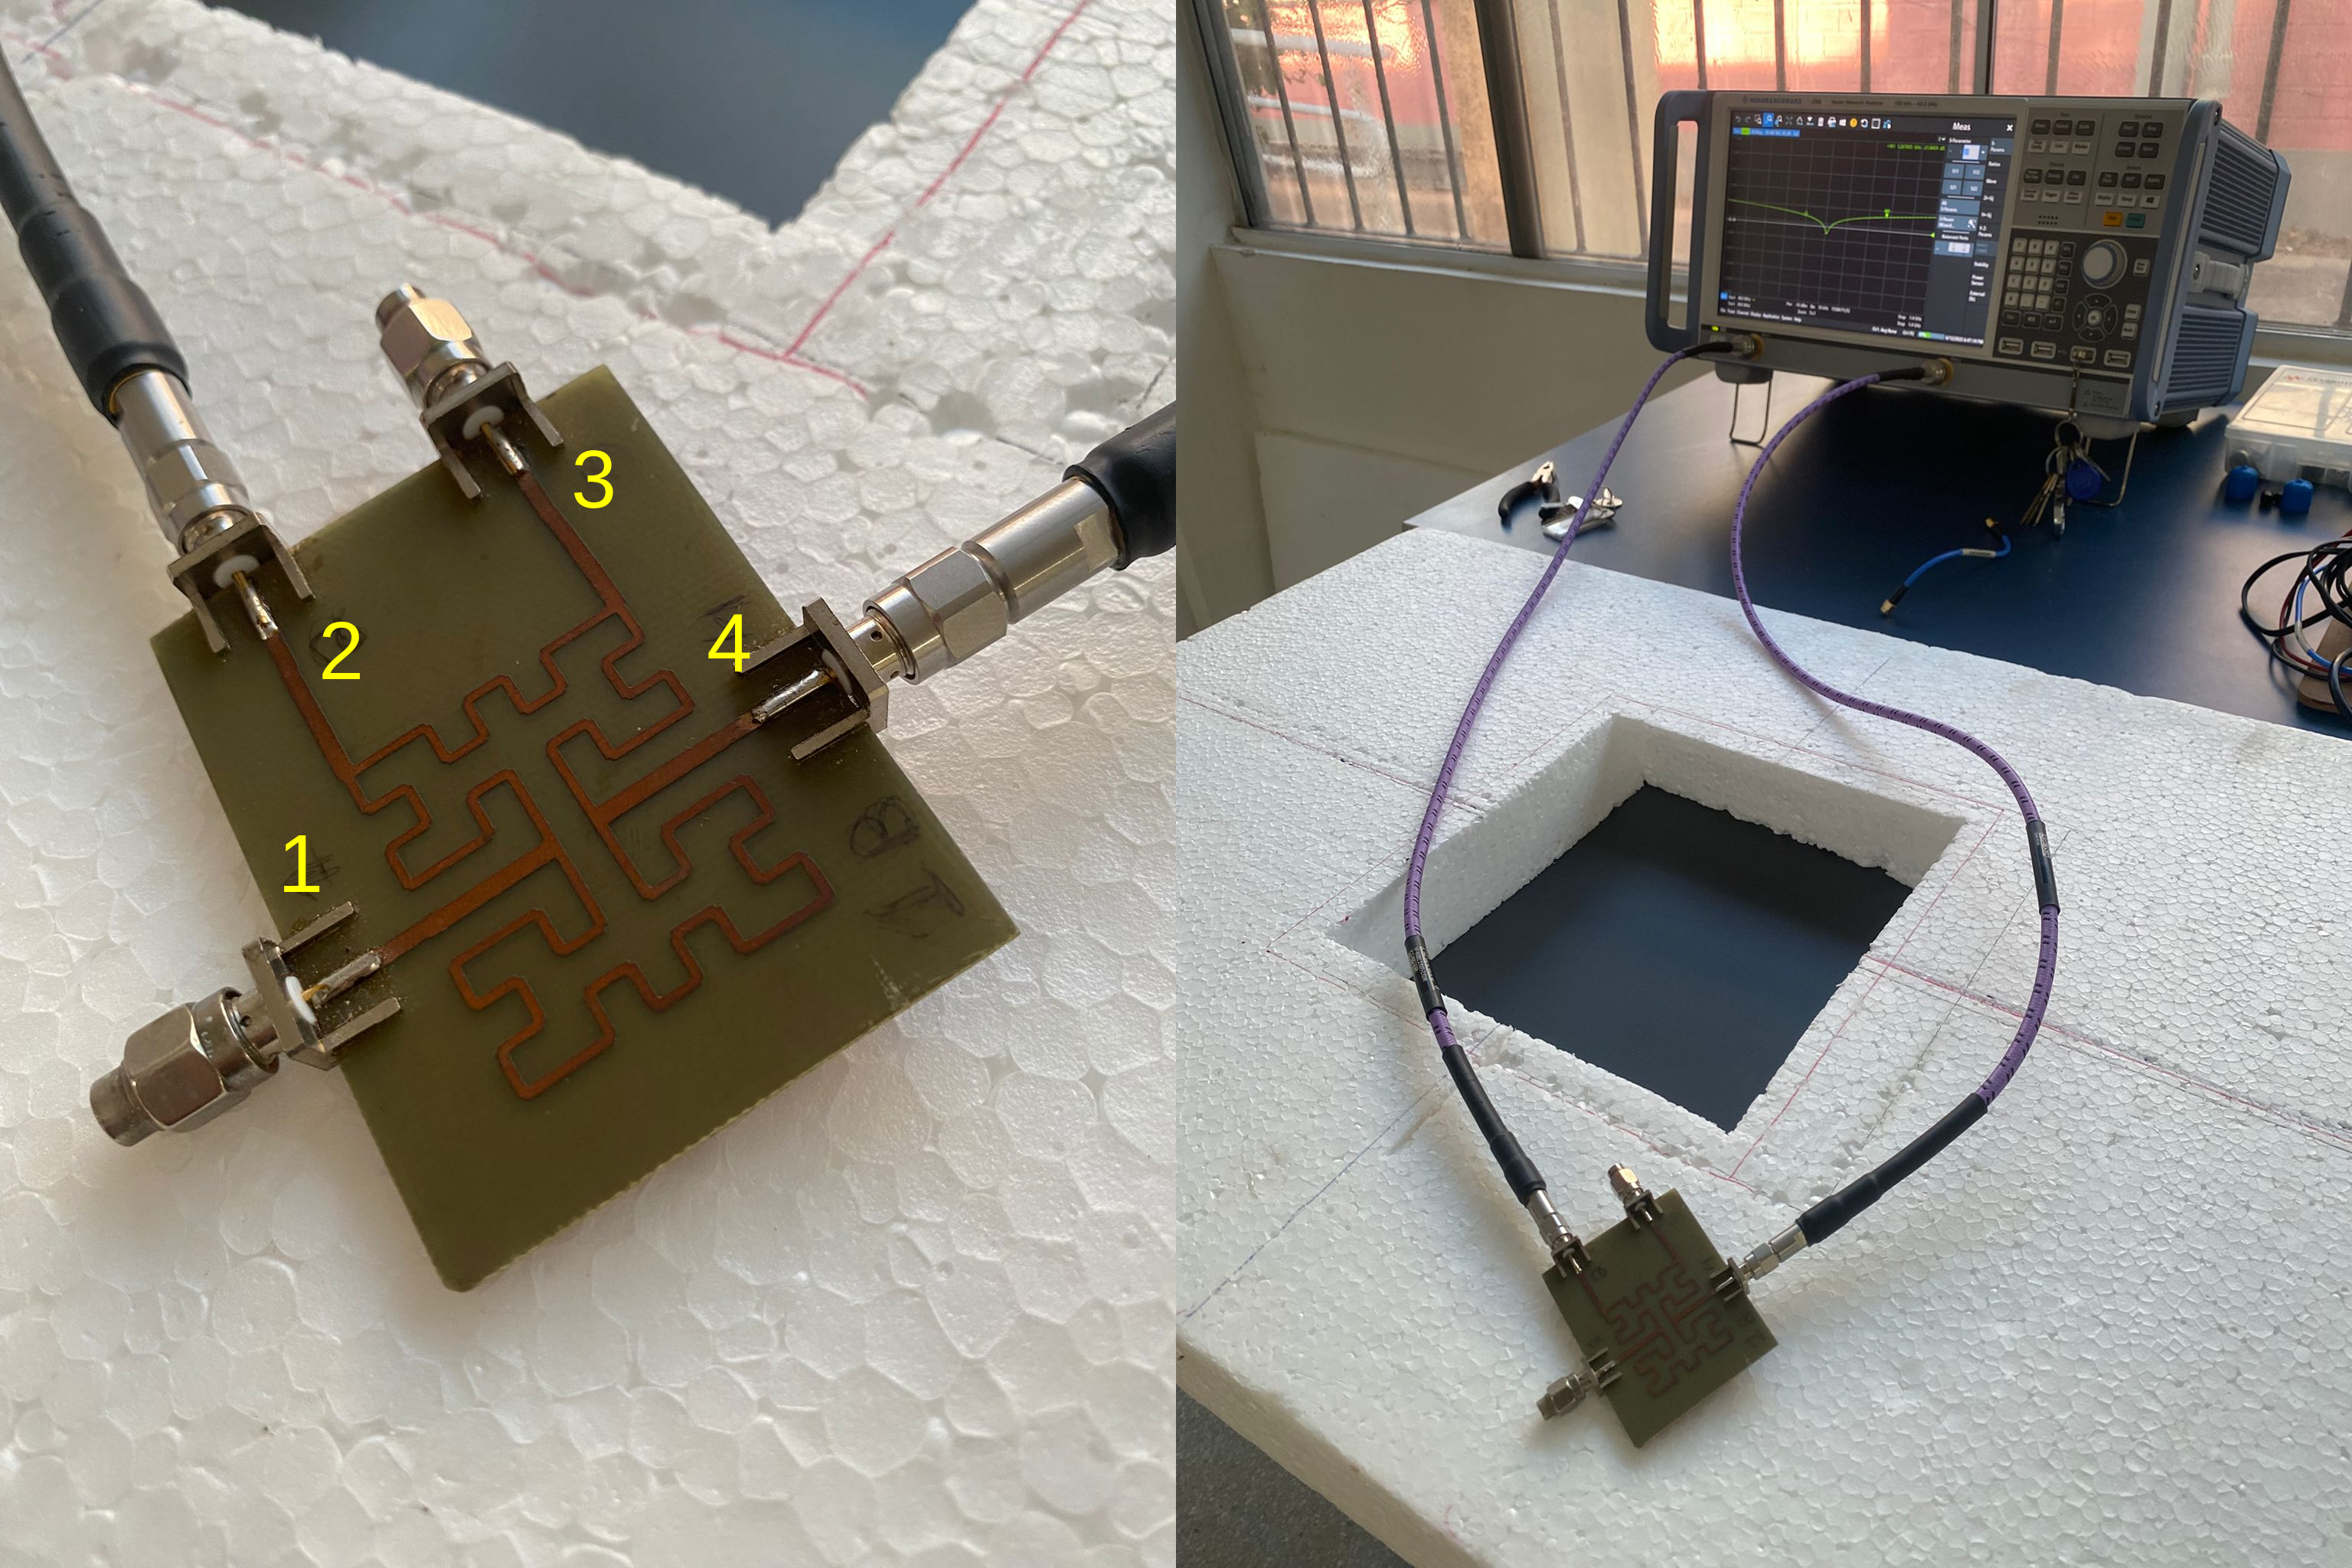
\includegraphics[width=0.5\textwidth]{fig/hybrid_receiver (1) (1).png}
    \caption{À esquerda: O híbrido fabricado na Universidade Federal de Campina Grande, onde as portas 1, 2, 3 e 4 são indicadas pelos números amarelos.À direita: A medição do parâmetro $S_{21}$ do híbrido usando o VNA Rohde \& Schwarz. As portas de entrada devem ser necessariamente alternadas—ou apenas pares ou apenas ímpares, seguindo esta numeração. O isolamento está presente apenas entre estas portas específicas. Portanto, temos as portas de entrada 2 e 4 e as portas de saída soma $\Sigma$ (porta 3) e a porta de diferença $\Delta$ (porta 1).}
    \label{fig:hybrid_receiver}
\end{figure}

\begin{figure}[h]
    \centering
    \includegraphics[width=\textwidth]{fig/image (14) (1).png}
    \caption{Parâmetros $S_{21}$ e $S_{11}$ do acoplador híbrido. As respostas de $S_{21}$ para as portas 1–2 e 3–4 (ambas mostradas em azul) exibem comportamento semelhante, assim como as respostas para as portas 2–3 e 1–4 (ambas mostradas em vermelho).}
    \label{fig:hybrid_result}
\end{figure}

Outro componente chave do receptor Uirapuru é o acoplador híbrido (veja a Fig.\ref{fig:hybrid_receiver}). Este dispositivo permite a combinação de sinais, produzindo saídas de soma ($\Sigma$) e diferença ($\Delta$), como ilustrado no esquema da Fig.\ref{fig:receptor}. Realizamos várias medições, incluindo a análise do parâmetro $S$ do híbrido, mostrada na Fig.~\ref{fig:hybrid_result}. O isolamento é observado nas configurações de portas cruzadas (por exemplo, portas 1–3 e 2–4), enquanto a transmissão ocorre predominantemente entre pares de portas adjacentes, como 1–2, 2–3, 3–4 e 1–4.Portanto, temos as portas de entrada 2 e 4 e as portas de saída soma $\Sigma$ (porta 3 no painel esquerdo da Fig.\ref{fig:hybrid_receiver}) e a porta de diferença $\Delta$ (porta 1 no painel esquerdo da Fig.\ref{fig:hybrid_receiver}). Enquanto isso, o parâmetro $S_{11}$ permanece consistente em todas as portas.Realizamos as medições—incluindo a análise do parâmetro $S$ dos LNAs, filtro passa-banda tipo cavidade, isolador e híbrido, conforme mostrado nas Figs.~\ref{fig:uirapuru_rec} e \ref{fig:hybrid_receiver}.

Finalmente, quando conectamos o híbrido à parte central do receptor, conforme apresentado no esquema da Fig.\ref{fig:receptor}, os sinais passam por outro LNA (Amplificador de Baixo Ruído) da WanTcom antes de chegarem ao nosso conversor analógico-digital (ADC) e ao sistema de processamento digital de sinais, que é um SKARAB da Peralex\footnote{https://www.peralex.com/radio-astronomy/}.

\begin{figure}[h]
    \centering
    \includegraphics[width=0.5\textwidth]{fig/drone_photo.png}
    \caption{a) Drone com transmissor de rádio Baofeng BF-777s, b) Transmissor de rádio Retevis RT85, c) Drone sobrevoando a Uirapuru, d) Uirapuru vista de cima.}
    \label{fig:uirapuru}
\end{figure}

\quad Em primeiro lugar, para testar a capacidade de detecção do nosso sistema, a Fig.\ref{fig:uirapuru} exibe o equipamento básico utilizado para as medições. Os testes envolveram sinais controlados manualmente gerados por um transmissor montado em um drone (Fig.\ref{fig:uirapuru}a) com um rádio portátil (Fig.\ref{fig:uirapuru}b) para produzir Interferência de Radiofrequência (RFI) intencional. Para o transmissor montado no drone, a detecção de medição do terceiro harmônico do sinal de 400 MHz (ou seja, 1200 MHz) foi realizada usando a corneta Uirapuru (Fig.\ref{fig:uirapuru}c e d).

\begin{figure}[h]
    \centering
    \includegraphics[width=0.6\textwidth]{fig/drone_waterfall (2).png}
    \caption{a) Uirapuru e drone com transmissor de rádio Baofeng BF-777s (destacado pela seta vermelha), b) Uirapuru vista de 35 metros acima. c) (em baixo) Apresentamos o espectro e o waterfall do sinal transmitido pelo Baofeng BF-777s acoplado ao drone.}
    \label{fig:drone_waterfall}
\end{figure}
A Figura~\ref{fig:drone_waterfall} ilustra a configuração da medição. Na Fig.\ref{fig:drone_waterfall}a, a corneta Uirapuru é mostrada ao lado do drone—destacado com uma seta vermelha—voando a uma altitude de 35 metros com o transmissor a bordo. A Fig.\ref{fig:drone_waterfall}b fornece uma vista de cima da configuração do Uirapuru.Como visto na Fig.~\ref{fig:drone_waterfall}c (em baixo), o terceiro harmônico do sinal transmitido, centrado em 1200 MHz, é claramente visível tanto no espectro quanto no gráfico waterfall. Além disso, um sinal fraco da banda GPS L5 em 1176 MHz também é detectado.Apesar do grande número de canais FFT utilizados ($2^{15}$), a frequência central do firmware apresenta um comportamento irregular nesta faixa de frequência, provavelmente devido a artefatos de processamento FFT ou sinais de sincronização. No entanto, essas anomalias não afetam a integridade dos resultados gerais.A potência exibida é o logaritmo de base 10 da saída não calibrada do SKARAB (portanto, não possui uma unidade física). A frequência corresponde a uma largura de banda de 187,5 MHz, com frequência central em 1120 MHz.

Após a realização de testes utilizando sinais controlados manualmente a partir de um transmissor montado em um drone, começamos a observar sinais comuns no céu detectados pelo Uirapuru.

Conforme mencionado no parágrafo anterior, a Fig. \ref{fig:Spectrum_4s} mostra alguns sinais típicos observados durante um dia inteiro de monitoramento. A potência é representada como o logaritmo de base 10 da saída não calibrada, e a frequência abrange uma largura de banda de 187,5 MHz centrada em 1120 MHz, com correspondência na escala de decibel (dB).

Notavelmente, um forte sinal da banda GPS L5 em 1176 MHz é claramente visível, juntamente com sinais menores em torno de 1200 MHz. Estes sinais são caracterizados por uma aparência suave e um desvanecimento gradual, indicando a relativa aproximação e afastamento da fonte do sinal do ponto de vista da corneta Uirapuru.

\begin{figure}[h]
    \centering
    \includegraphics[width=0.8\textwidth]{fig/Spectrum_4s.png}
    \caption{Detecção de Sinais GPS L5 (1176 MHz) e 1200 MHz. O painel esquerdo mostra o espectro de potência com um forte sinal GPS L5 em 1176 MHz e um sinal mais fraco próximo a 1200 MHz. O painel direito exibe o correspondente waterfall plot (diagrama de cachoeira), onde o sinal L5 aparece fraco no início e aumenta em intensidade.
}
    \label{fig:Spectrum_4s}
\end{figure}

A Figura \ref{fig:uirapuru_waterfall} apresenta um dia completo de observação do Uirapuru, correspondente a 9 de maio de 2025. A potência exibida é o logaritmo de base 10 da saída não calibrada do Skarab, com correspondência na escala de decibel (dB).

A frequência abrange uma largura de banda de 187,5 MHz, variando de 1026,25 MHz a 1213,75 MHz, e o período de observação cobre de 00:00 a 23:59 do mesmo dia. A figura revela a passagem de satélites GPS, com sinal visível na banda L5. Adicionalmente, entre 10:00 e 15:00—aproximadamente o meio-dia—é observado um provável trânsito solar em toda a faixa de frequência.

\begin{figure}
    \centering
    \includegraphics[width=1.0\linewidth]{fig/Waterfall_1day_2025_05_09.png}
    \caption{TOD (Dados Ordenados por Tempo) de observação do Uirapuru para o dia 2025-05-09 em 24 horas. No eixo $y$ são apresentados os canais de frequência em MHz, no eixo $x$ é apresentado o tempo em horas, e o logaritmo de base 10 da intensidade (potência não calibrada) é apresentado pela barra de cores, onde definimos o valor máximo como três para investigar as informações principais.}
    \label{fig:uirapuru_waterfall}
\end{figure}

\section{Agradecimentos}
\quad O progresso detalhado neste trabalho foi significativamente impulsionado pelo ambiente colaborativo da colaboração BINGO, a quem expresso minha gratidão. Agradecimentos especiais são dirigidos às equipes técnicas do LABMET, sob a coordenação dos Professores Edmar Gurjão e Amilcar Queiroz, e ao INPE pelo apoio contínuo e por disponibilizar a infraestrutura de teste e a expertise essenciais. Estendo também meu reconhecimento à FAPESQ-PB pelo seu valioso apoio à pesquisa e ao desenvolvimento no estado da Paraíba.

\appendix
\section{Instalação e Execução do \textit{casperfpga}}
\label{appendix:casperfpga}

\quad O pacote casperfpga é responsável pelo primeiro contato com a SKARAB. A partir dele, é possível utilizar arquivos .fpg já existentes e testar as funcionalidades da placa via Python 2.7, por meio do terminal do computador. Os testes realizados tiveram como objetivo verificar o desempenho do Python 2.7 com a SKARAB, e os resultados foram satisfatórios. Para utilizar a plataforma, é necessário seguir alguns passos para instalar o casperfpga em um ambiente Python 2.7. A seguir, são apresentados os procedimentos para instalar o casperfpga do zero no Ubuntu 16.04.

\subsection{Instalação do \textit{casperfpga}}

\begin{enumerate}
    \item Instale o Python 2.7:
    \begin{verbatim}
    sudo apt install python2.7
    \end{verbatim}
    
    \item Instale o \texttt{virtualenv} para criar ambientes virtuais:
    \begin{verbatim}
    sudo apt install virtualenv
    \end{verbatim}
    
    \item Crie um ambiente virtual:
    \begin{verbatim}
    virtualenv -p python2 cfpga_venv
    \end{verbatim}
    
    \item Ative o ambiente virtual:
    \begin{verbatim}
    source cfpga_venv/bin/activate
    \end{verbatim}
    
    \item Instale o \texttt{git}:
    \begin{verbatim}
    sudo apt install git
    \end{verbatim}
    
    \item Clone o repositório da CASPER:
    \begin{verbatim}
    git clone https://github.com/casper-astro/casperfpga
    \end{verbatim}
    
    \item Entre no repositório da CASPER:
    \begin{verbatim}
    cd casperfpga
    \end{verbatim}
    
    \item Instale alguns requerimentos:
    \begin{verbatim}
    sudo apt install build-essential && sudo apt install python-dev
    \end{verbatim}
    
    \item Instale os requerimentos do \texttt{casperfpga}:
    \begin{verbatim}
    pip install -r requirements.txt
    \end{verbatim}
    
    \item Entre na pasta \texttt{progska}:
    \begin{verbatim}
    cd progska
    \end{verbatim}
    
    \item Compile o \texttt{progska}:
    \begin{verbatim}
    make
    \end{verbatim}
    
    \item Volte para a pasta \texttt{casperfpga}:
    \begin{verbatim}
    cd ..
    \end{verbatim}
    
    \item Instale o pacote \texttt{casperfpga}:
    \begin{verbatim}
    pip install .
    \end{verbatim}
    
    \item Saia da pasta \texttt{casperfpga}:
    \begin{verbatim}
    cd ..
    \end{verbatim}
    
    \item Instale o \texttt{matplotlib}:
    \begin{verbatim}
    pip install matplotlib
    \end{verbatim}
    
    \item Instale ferramentas de rede:
    \begin{verbatim}
    sudo apt install net-tools
    \end{verbatim}
    
    \item Vá em configurações de internet (\textit{Network Settings}) e configure:
    \begin{itemize}
        \item “Compartilhado para outros computadores” (\textit{Shared to other computers}) para o IPv4;
        \item “Ignore” para o IPv6.
    \end{itemize}
    
    \item Configure o MTU para 9000 em “Identidade” (\textit{Identity}) e reinicie a conexão 40GbE após esses passos.
    
    \item Para testar, cheque o IP da SKARAB com conexão 40GbE:
    \begin{verbatim}
    arp -a
    \end{verbatim}
    No exemplo, observamos:
    \begin{verbatim}
    (10.42.0.201) at 06:50:02:0f:02:01 [ether] on enp1s0f0
    \end{verbatim}
\end{enumerate}

\subsection{Execução na IDE \textit{IPython}}

Após todos esses passos, a SKARAB pode ser operada por meio da IDE \textit{IPython}:

\begin{enumerate}
    \item Execute o \textit{IPython} (IDE utilizada para operar a SKARAB):
    \begin{verbatim}
    ipython
    \end{verbatim}
    (sempre execute com o ambiente Python ativado).

    \item Dentro da IDE \textit{IPython}, importe o módulo \texttt{casperfpga}:
    \begin{verbatim}
    import casperfpga
    \end{verbatim}

    \item Verifique a versão instalada do \texttt{casperfpga}:
    \begin{verbatim}
    casperfpga.__version__
    \end{verbatim}
    (observe que são dois sublinhados “\_” antes e depois da palavra \texttt{version}, sem espaços).

    \item Estabeleça a conexão com a SKARAB:
    \begin{verbatim}
    fpga = casperfpga.CasperFpga('10.42.0.201')
    \end{verbatim}

    \item Faça o upload do seu arquivo \texttt{.fpg} para a SKARAB:
    \begin{verbatim}
    fpga.upload_to_ram_and_program('file.fpg')
    \end{verbatim}
\end{enumerate}

\section{Instalação e Execução do \textit{mlib\_devel}}
\label{appendix:mlib_devel}

\quad Responsável pela criação de arquivos ".fpg" de autoria própria através do MATLAB R2018a e do Vivado 2019.1 no Ubuntu 16.04. Isso nos permite programar a SKARAB para realização de diversas atividades. Para isso, seguimos com os seguintes passos.

\begin{enumerate}
    \item Instalação de Dependências Básicas:
    %\begin{verbatim}
    
    Antes de iniciar a instalação do Vivado, é essencial garantir que o sistema possua bibliotecas e pacotes fundamentais. Esses pacotes são necessários para assegurar que o software funcione corretamente, sem conflitos de bibliotecas ou dependências ausentes.
    %\end{verbatim}

    \begin{enumerate}
        \item Biblioteca padrão C++

        - Comando: \begin{verbatim}
            sudo apt-get install libstdc++6
        \end{verbatim}

        Explicação: A biblioteca C++ é necessária para a execução de diversos componentes do Vivado, que dependem de código escrito nesta linguagem.

        \item Biblioteca GTK+ 2.0

        - Comando: \begin{verbatim}
            sudo apt-get install libgtk2.0-0
        \end{verbatim}

        Explicação: A GTK+ é usada para criar interfaces gráficas e é crucial para garantir que o Vivado e outras ferramentas que usam GUI funcionem corretamente.

        \item Ferramentas de desenvolvimento dpkg

        - Comando: \begin{verbatim}
            sudo apt-get install dpkg-dev
        \end{verbatim}

        Explicação: O dpkg é o sistema de gerenciamento de pacotes do Ubuntu e suas ferramentas de desenvolvimento são necessárias para compilar ou instalar alguns dos pacotes do software Xilinx.

        \item Instalação de Python e Pip

        - Comando: \begin{verbatim}
            sudo apt install python3-pip
        \end{verbatim}
        \begin{verbatim}
            sudo apt install python-dev
        \end{verbatim}

        Explicação: Python é frequentemente utilizado para scripts de automação no ambiente de desenvolvimento, e o Pip permite gerenciar pacotes e bibliotecas python.

        \item Bibliotecas de terminal e ncurses

        - Comando: \begin{verbatim}
            sudo apt install libtinfo5 libncurses5
        \end{verbatim}

        Explicação: Essas bibliotecas são usadas para lidar com a interface de linha de comando e são exigidas por vários programas no ambiente Linux.

        \item Adicionar suporte ao Qtf4 para a interface gráfica

        - Comando: \begin{verbatim}
            sudo add-apt-repository ppa:rock-core/qt4
        \end{verbatim}

        Explicação: Algumas ferramentas gráficas do Vivado utilizam o framework Qt4, tornando a instalação dessas bibliotecas necessária para uma correta exibição de janelas.

        \item Instalar bibliotecas Qt4

        - Comando: \begin{verbatim}
            sudo apt update
            sudo apt install libqtcore4 libqtgui4
        \end{verbatim}

        Explicação: As bibliotecas Qt4 são responsáveis por fornecer os componentes visuais da interface gráfica do usuário.
    \end{enumerate}

    \item Instalação do \textbf{MATLAB R2018a}:

    \begin{enumerate}
        \item Baixe o MATLAB R2018a na página da Mathworks.
        \item Após baixar o MATLAB R2018a, vá para o caminho onde está o instalador:
        \begin{verbatim}
            cd /caminho/para/matlab/download/matlab_R2018a_glnxa64.zip
        \end{verbatim}
        \item Crie uma pasta para o MATLAB:
        \begin{verbatim}
            mkdir matlab_R2018a
        \end{verbatim}
        \item Descompacte o .zip:
        \begin{verbatim}
            matlab_R2018a_glnxa64.zip -d matlab_R2018a
        \end{verbatim}
        \item Entre na pasta:
        \begin{verbatim}
            cd matlab_R2018a
        \end{verbatim}
        \item Instale o MATLAB
        \begin{verbatim}
            sudo ./install
        \end{verbatim}
        \item Após a instalção, execute o MATLAB. Digite o seguinte comando:
        \begin{verbatim}
            .matlab
        \end{verbatim}
        dentro da pasta /path/to/MATLAB/R2018a/bin \\ (no nosso caso: /usr/local/MATLAB/R2018a/bin/).
    \end{enumerate}
    
    \item Instalação do \textbf{Vivado 2019.1}:
    Após garantir que o sistema possui todas as dependências básicas, a instalação do Vivado pode ser feita com segurança. Seguem os passos:

    \begin{enumerate}
        \item Baixe .zip para instalação do Vivado 2019.1 no site da Xilinx. Após isso descompacte o arquivo no formato .tar.gz:
        - Comando:
        \begin{verbatim}
            tar -xvzf Xilinx_Vivado_SDK_2019.1_0524_1430.tar.gz
        \end{verbatim}

        \item Entre na pasta descompactada.
        - Comando:
        \begin{verbatim}
            cd Xilinx_Vivado_SDK_2019.1_0524_1430
        \end{verbatim}

        \item Inicie o instalador.
        - Comando:
        \begin{verbatim}
            sudo ./xsetup
        \end{verbatim}

        \item Marque a opção "Vivado HL System Edition"

        \item Também marque a opção: check "Vivado Design Suite" on "Design Tools"

        \item Após a instalação completa, execute o Vivado para testar com o comando
        \begin{verbatim}
            sudo ./vivado
        \end{verbatim}
        dentro da pasta /tools/Xilinx/Vivado/2019.1/bin

        \item Gere uma licença Vivado, a opção gratuita tem duração de 30 dias. Para inserir a licença, clique em "Help" e "Manage License" dentro do Vivado.

        \item Outros comandos podem ser necessários para executar o Vivado adequadamente:

        \begin{enumerate}
            \item 
            sudo cp -r $\sim$/Downloads/Xilinx.lic /home/bingo/.Xilinx/

            \item sudo cp -r $\sim$/Downloads/Xilinx.lic /tools/Xilinx/Vivado/2019.1/data/sysgen/ \\ hwcosim\_compiler/pp\_ethernet/

            \item sudo cp -r $\sim$/Downloads/Xilinx.lic /tools/Xilinx/Vivado/2019.1/data/ip/core\_licenses/
        \end{enumerate}
    \end{enumerate}

    \item Instalação do \textbf{Vitis} 

    O Vitis é a plataforma unificada da Xilinx para o desenvolvimento de sistemas heterogêneos. Para instalá-lo:

    No Vivado, vá até o menu "Help" e selecione "Add Design Tools or Devices" para integrar o Vitis ao ambiente de desenvolvimento.

    \item Configuração do Ambiente Python

    \begin{enumerate}
        \item Instalar o pacote python3-venv:
        \begin{verbatim}
            sudo apt install python3-venv
        \end{verbatim}
        \item Criar e ativar um ambiente virtual
        \begin{verbatim}
            python3 -m venv casper_venv (para criar)
        \end{verbatim}
        \begin{verbatim}
            source casper_venv/bin/activate (para ativar)
        \end{verbatim}
        Explicação: O ambiente virtual garante que todas as bibliotecas específicas para o projeto estejam isoladas.
    \end{enumerate}

    \item Instalação do toolflow \textit{mlib\_devel}
    O mlib\_devel é um toolbox do MATLAB/Simulink utilizado para instanciar blocos e pacotes desenvolvidos pela colaboração CASPER, facilitando o projeto e a integração de sistemas digitais em FPGAs.

    \begin{enumerate}
        \item Clonar o repositório:
        \begin{verbatim}
            git clone -b master https://github.com/peralex/mlib_devel
        \end{verbatim}
        \item Entre na pasta mlib\_devel:
        \begin{verbatim}
            cd mlib_devel
        \end{verbatim}
        \item Adicione os seguintes requeriments no arquivo requirements.txt
        \begin{verbatim}
            numpy < 1.9
            colorlog
            pyaml
            odict
            #xml2vhdl requirements
            lxml==4.3.0
            pyyaml==3.13
            -e
            git+http://github.com/casper-astro/
            xml2vhdl#egg=xml2vhdl_ox-0.2.2-py3.5.egg
            &subdirectory=scripts/python/xml2vhdl-ox
        \end{verbatim}
        \item Antes de instalar os requerimentos, instale o python3-dev:
        \begin{verbatim}
            sudo apt install python3-dev
        \end{verbatim}
        \item Instale agora os requerimentos para o mlib\_devel:
        \begin{verbatim}
            pip3 install -r requirements.txt
        \end{verbatim}
    \end{enumerate}

    \item Configure o arquivo startsg.local.example. Coloque as seguintes linhas dentro do arquivo
    \begin{verbatim}
        export XILINX_PATH=/tools/Xilinx/Vivado/2019.1
        export MATLAB_PATH=/usr/local/MATLAB/R2018a
        export PLATFORM=lin64
        export JASPER_BACKEND=vivado
        export LD_PRELOAD=${LD_PRELOAD}:"/usr/lib/x86_64-linux-gnu/libexpat.so"
        export CASPER_PYTHON_VENV_ON_START=/home/bingo/casper_venv
    \end{verbatim}

    \item Execute o mlib\_devel usando o ambiente python3:
    \begin{verbatim}
        ./startsg startsg.local.example
    \end{verbatim}
    No nosso caso, temos a seguinte expressão no terminal:
    \begin{verbatim}
        (casper_venv) bingo@bingo:~/mlib_devel$ ./startsg startsg.local.example
    \end{verbatim}

\end{enumerate}



\begin{thebibliography}{00}

\bibitem{melis2024skarab}Melis, A., Cabras, A., Comoretto, G., Concu, R., Fiorentini, M., Ladu, A., Maccaferri, A., Migoni, C., Murgia, M., Pilia, M. \& Others The SKARAB Board in the Framework of Single-Dish Radio Astronomy.  (2024),

\bibitem{wuensche2021baryon}Wuensche, C., Abdalla, E., Abdalla, F. \& Others Baryon Acoustic Oscillations from Integrated Neutral Gas Observations: an instrument to observe the 21cm hydrogen line in the redshift range 0.13 < z < 0.45–status update. {\em Anais Da Academia Brasileira De Ciências}. \textbf{93} pp. e20201096 (2021)

\end{thebibliography}

\end{document}